\documentclass[lang=cn,10pt]{elegantbook}

\title{给孩子的语文书之何以中国}
\subtitle{LaTeX 经典之作}

\author{齐齐爸}
\institute{共同进步组织}
\date{June 9, 2026}
\version{0.1}
\bioinfo{自定义}{语文寄语}

\extrainfo{不要以为抹消过去，重新来过，即可发生什么改变。—— 比企谷八幡}

\setcounter{tocdepth}{3}

\logo{logo-blue.png}
\cover{cover.jpg}

% 本文档命令
\usepackage{array}
\newcommand{\ccr}[1]{\makecell{{\color{#1}\rule{1cm}{1cm}}}}

\usepackage{graphicx}   % 图片插入
\usepackage{subcaption}
\usepackage{geometry}
\geometry{a4paper, margin=2.5cm}

\usepackage{indentfirst}  % 强制首段也缩进

% 设置段首缩进为2个汉字宽度
\setlength{\parindent}{2em}

% 修改标题页的橙色带
% \definecolor{customcolor}{RGB}{32,178,170}
% \colorlet{coverlinecolor}{customcolor}

%新增
\usepackage{tabularx}            % 自动换列表格
\usepackage{booktabs}            % 三线表
\newcolumntype{L}{>{\raggedright\arraybackslash}X}  % 左对齐自动换列


\begin{document}

% 在正文开始处再强制设置一次
\setlength{\parindent}{2em}

\maketitle
\frontmatter

\tableofcontents

\mainmatter

\chapter{病句辨析与修改}

\begin{introduction}
  \item 搭配不当
  \item 用词不当
  \item 语序不当
  \item 成分残缺
  \item 成分赘余
  \item 结构混乱
  \item 不合逻辑
  \item 表意不明
\end{introduction}


\section{主要类型知识归纳}

\subsection{搭配不当}

\subsubsection{主谓搭配不当}

例：他一进教室，同学们的眼睛都集中到他的身上。

解析：句中主语“眼睛”与谓语“集中”搭配不当。“眼睛”不能“集中”，应改为“目光”。

\subsubsection{动宾搭配不当}

例：英雄们把红旗和胜利插上了敌人的阵地。

解析：句中动宾搭配不当，“红旗”可以插，“胜利”怎么插？应改为“英雄们把胜利的红旗插上了敌人的阵地”。

\subsubsection{主宾搭配不当}

例：冬天的上海是美丽的季节。

解析：本句提取主干为“上海是季节”，“冬天”是“季节”，“上海”不是“季节”，应改为“上海的冬天是美丽的季节”。

\subsubsection{修饰语和中心语搭配不当}

例：我们有一双聪明能干的手，什么造不出来？

解析：本句属于修饰语和中心语搭配不当。“聪明”不能修饰“手”，应把“聪明”改为“灵巧”。

\subsubsection{一面与两面搭配不当}

例：摄影作品拍得好坏，诗歌写得有味无味，是由一个人的思想、艺术修养决定的。

解析：句中“思想、艺术修养”的含义是确定的，意思是“有思想、艺术修养”，只能与前面的“拍得好”、“写得有味”意思搭配。这个句子要做到前后搭配，需要在“思想、艺术修养”后加“高低”一词。

\subsection{用词不当}

\begin{enumerate}[leftmargin=*]
    \item 感情色彩不当。如：他认真刻苦的学习精神，值得我们每个同学效尤。（“效尤”含贬义，可改为“学习”）
    \item 关联词使用不当。如：只要坚持下去，我们才能取得成功。（关联词语一般成对使用，“只要”一般与“就”搭配，“只有”与“才”搭配。）
    \item 意思表达不当。如：他这个人，性格直爽，为人忠厚，说起话来信口开河。（“信口开河”意为“随口乱说一气”，此处误用为“快言直语”。）
    \item 词性误用。如：从大量统计资料来看，吸烟能导致癌症是无可疑问的。（“疑问”是名词，应改为“置疑”。）
    \item 大词小用。如：每个老师日常从事的事业，是平凡而又伟大的。（“事业”应改为“工作”。）
\end{enumerate}

\subsection{语序不当}

\subsubsection{名词修饰语次序不当}

例：在新中国的建设事业中，他们发挥着无穷的蕴藏着的力量。

解析：“无穷的”应紧靠“力量”。多项定语与中心语的正确次序一般是：（1）表领属性的或时间、处所的；（2）指称或数量的短语；（3）动词或动词短语；（4）形容词或形容词短语；（5）名词或名词短语。另外，带“的”的定语放在不带“的”的定语前。

\subsubsection{动词修饰语次序不当}

例：开考半个小时后，就有人陆续交卷。

“陆续”应移到“有”的前面。多项状语次序比较复杂，须特别注意的是：（1）先时间后处所；（2）先介词结构后动词、形容词；（3）表示对象的介词结构一般紧靠中心语；（4）不要弄错修饰对象。

\subsubsection{关联词语位置不当}

例：他如果不能实事求是，事业就会受到损失。

解析：“他”应移到“如果”后面。一般来说，两个分句同一个主语时，关联词语在主语后边；不同主语时，关联词语在主语前边。

\subsection{成分残缺}

\subsubsection{缺少主语}

例：通过形式多样的活动，使广大青年学生树立了正确的人生观和价值观。

解析：“通过”与“形式多样的活动”构成介宾短语，充当状语，后一分句由“使”领起，造成该句缺少主语，“通过”或“使”保留一个即可。

\subsubsection*{缺谓语}

例：中国人民正在为建设一个现代化的社会主义强国。

“为建设一个现代化的社会主义强国”是个介词结构，只能作状语而不能作谓语。“为建设强国”怎么样？话没说完。在“强国”后面补上“而努力奋斗”，句子就有谓语了。

\subsubsection{缺少宾语中心语}

例：经过阿富汗与伊拉克战争，美国得出无须依靠大型军事基地也可以打赢一场战争。

解析：此句缺少宾语中心语，“得出”与“打赢一场战争”不能搭配，应在“战争”后面加上“的结论”。

\subsubsection{缺介词}

例：周日，嘉成老师跟他关系最好的宏涛老师去逛街了。

乍看好像没什么问题，分析一下句子成分会发现“跟他关系最好的”是修饰“宏涛老师”的定语成分，而这里想表达的是“嘉成老师和宏涛老师”去逛街了。若要修改，在“跟”字前加个“和”即可。

\subsection{成分赘余}

成分赘余，顾名思义就是句子里有多余的成分，造成了语义重复的问题。

\subsubsection{主语有多余成分}

例：全场座位座无虚席，教授的报告赢得了同学们的热烈掌声。

“座无虚席”的“座”已经是“座位”的意思了，没有必要再说一次“座位”。

\subsubsection{谓语有多余成分}

例：这位老教授的学术造诣在国内可以堪称一流。

“堪”的意思就是可以、能够，再说一个“可以”，说重了。可以改成“在国内堪称一流”或者“在国内可以称得上一流”。

\subsubsection{宾语有多余成分}

例：只有密切接触社会，联系群众，才能对国家安危和人民快乐提出具有真知灼见的意见。

“真知灼见”的“见”就是意见的意思，这里直接说“提出真知灼见”就行了，没必要加“的意见”。

\subsubsection{定语多余}

例：你去劝劝她，让她别把过去的往事放在心上。

“往事”的“往”就是“过去”的意思，“过去的往事”，显然说重复了，可以说“别把往事放在心上”，或者“别把过去的事情放在心上”。

\subsubsection{状语多余}

例：在使用电器的时候，如果一旦出现漏电现象，应该立即切断电源。

“如果”和“一旦”都是表示假设，没有必要都用，删去任意一个即可。

\subsubsection{其他多余}

例：从那以后，这个原本平静的家里，不时发生使人不安的怪事出来。

句中的“发生”就有“出来”的意思，再加“出来”就多余了，形成了补语赘余的问题，应当删掉“出来”。

\subsection{结构混乱}

\subsubsection{一个句子套用了两种结构}

例：一个人变好变坏，关键在于内因起决定作用。

“关键在于内因”与“内因起决定作用”保留一个即可。

\subsubsection{两个分句糅成一个单句}

指本来是两个分句组成的复句，却被杂糅成一个单句。

例：小张除跳舞外，兼任报幕、开场、结尾的节目还得由她编导。

“小张……兼任报幕”和“开场……由她编导”是两个分句，各有主语，其间误用顿号；“兼任”一词一直管到“节目”，造成杂糅和搭配不当的双重毛病。

\subsubsection{藕断丝连}

指一句话结构已完整，却把它的最后部分用作另一部分的开头。

例：处理好人与自然的关系，要靠政府的力量，同时也不能不发挥民间力量在舆论动员、监督检查等方面起到无可替代的作用。

“民间力量”在前部分作宾语，整个句子已经完整，但加上“在舆论……的作用”部分，又使它作了后部分的主语，整个句子的结构乱了。为突出“民间力量”，可从它后面断开，再在“在舆论……的作用”前加“民间力量”，使整个句子变成两句话。

\subsubsection{中途易辙}

一句话说了一半，忽然另起炉灶，重来一句。

例：观摩了这次关于农村经营承包合同法的庭审以后，对我们这些“村官”的法律水平有了很大的提高。

“观摩……庭审”的主语无疑是“我们”（省略了），但接下来的“对我们……的主语”显然不是“我们”，中途更换主语造成了结构混乱，删去“对”。

\subsection{不合逻辑}

\subsubsection{自相矛盾}

例：他是多少个死难者中幸免的一个。

解析：既然“幸免”，自然是没有死，怎么能说是“死难者中的一个”呢？应改为“多少人遇难了，他是幸免的一个”。

\subsubsection{并列不当}

例：他们一面拼命地往上爬，一面又不免跌落深渊。

解析：“一面……一面……”表示两件事同时进行，句中的两件事显然不是同时的，应改为“他们虽然拼命地向上爬，但是最终不免跌落深渊”。

\subsubsection{强加因果}

例：最近我这位朋友去了一趟南方回来，结果他的思想依然如故。

解析：去了南方回来思想变了，可以说是去了一趟南方的结果，现在“思想依然如故”，怎么能说是去了一趟南方的“结果”呢？

\subsubsection{主客体颠倒}

例：他从小在这长大，这里的山山水水，对他太熟悉了。

解析：“山山水水”是客观存在，是“熟悉”的客体，“他”是“熟悉”的主体。这句话正确的说法应该是“他从小在这长大，对这里的山山水水，他太熟悉了”。

\subsection{表意不明}

\subsubsection{指代不明}

如：有人主张接受，有人反对，他同意这种主张。（这种主张到底是指接受还是反对，交代不清。）

\subsubsection{介词误用}

如：奥斯特洛夫斯基的《钢铁是怎样炼成的》对于中国青年是不陌生的。（主体是人，客体是物，即作品，应是人对物不陌生。）

\section{二、常见的辨析病句的方法}

\begin{enumerate}[leftmargin=*]
    \item \textbf{紧缩法}：这是最常用的语法分析方法。先把句中的附加成分（定语、状语和补语）都去掉，紧缩出主干，检查主干是否存在成分残缺、搭配不当的语病；如果主干没问题，再检查局部，看修饰语和中心语之间的搭配有无问题，修饰语的内部是否存在语序问题。
    \item \textbf{逻辑分析法}：有的语病从语法上不好找毛病，就得从事理上进行分析，这就是逻辑意义分析法。逻辑意义分析法要从概念、判断、推理方面考虑是否得当，从句句的前后顺序、句间关系、关联词语的使用等方面考虑是否合适。例如：“该市有人不择手段伪造伪劣产品。”此句“伪造伪劣产品”是不合事理的，应改为“制造伪劣产品”或“伪造名牌产品”。辨析病句还得从语言习惯、感情色彩、语体色彩等方面仔细推敲，逐一分析，就能辨其正误，识其病因。
    \item \textbf{语感审读法}：调动语感，在审读的过程中，从感性上察觉语句的毛病。即按习惯的说法看是否别扭。如别扭则再作分析比较，辩明原因，加以修改。
    \item \textbf{造句类比法}：对句子的毛病拿捏不准时，按原句格式仿造一些浅近的、容易把握的句子加以比较，就能比较清楚地看到语病所在。
    \item \textbf{修改病句的原则}：
        \begin{itemize}
            \item 不要改变句子的原意。
            \item 修改后不能再出现新的语病。
            \item 要保持句子的简洁。
            \item 要根据实际表达需要修改，不能为了改病句而改病句，改动的字数要尽量少。切忌违背原意，另起炉灶，按自己的意志另选一个句子去代替原句。
        \end{itemize}
\end{enumerate}

\section{考场练兵}

\subsection{下列句子中，没有语病的一项是（\ ）}

A. 滥用外来语，既消解了中国文化精深而丰富的内涵，也影响了汉语表意功能的发挥。

B. 学校能否把素质教育的功夫做实，关键在于将考试建立在发展素质教育的基础上。

C. 今年，文化和旅游部继续开展“云游非遗”线上推广活动，鼓励人们走进传统文化、发现非遗之美。

D. 假如你是一粒种子，尽管是生在沃野，还是长在峭壁，都要坚强地扎根生长。


\subsection{下列病句修改不正确的一项是（\ ）}

A. 第12版《新华字典》收录了“拼购”“刷屏”等网络词语，意味着一些网络词语被更广泛地使用和接受。（将“使用和接受”改为“接受和使用”）

B. 党的十八大以来，我国推动生态环境保护之大前所未有，环境污染防治行动成效明显。（将“明显”改为“显著”）

C. 有识之士认为，能否科学设计家庭作业是实现家校良性互动、家庭作业回归育人本位的重要条件之一。（删去“否”）

D. 贯彻落实中央文化润疆精神，就要努力创作展现兵团精神的更多新时代文艺作品。（将“更多”调到“创作”之后）



\subsection{下列对病句的修改不正确的一项是（\ ）}

A. 人行道的一手扶扶，朋友间的一份鼓励，对手间的一丝宽容……这件件微薄的善举，让我内心感到由衷的温暖。（删去“由衷的”）

B. 由于采用了科学的复习方法，他的学习效率有了较大幅度的改动。（将“改动”改为“改变”）

C. 在阅读名著中，使我们明白许多做人的道理，悟出人生的真谛。（去掉“在……中”）

D. 时代的进步要求人们开阔的视野，创新的思维。（在“人们”后加“具有”）



\subsection{下列表述不正确的一项是（\ ）}

A. 文言文中的称谓语非常丰富，有自称，有对他人的爱称，敬称等。如“卿今当涂掌事”中的“卿”是古代君对臣的爱称。

B. 《卖油翁》选自《归田录》卷一，作者欧阳修，号醉翁，晚号六一居士，谥号文忠，北宋政治家、文学家，唐宋八大家之一。

C. 汉字在这些国家的应用与传播，提升了民族文化的交流，成为中国与世界各国友谊的桥梁。（该句有语病，应把“提升”改为“提高”）

D. “沿河边（跑步）”和“从昨天（开始）”中的加着重号的词都是介词，它们跟名词或代词结合在一起组成短语，表示地点、时间等。



\subsection{下列句子中没有语病、表达清楚的一项是（\ ）}

A. 环境很艰苦，条件很困难，只有我们坚定信心，顽强不屈，才能迎来人生的绿洲。

B. 王继才在孤岛上坚守32年，把最美好的年华全部献给祖国的海防事业。

C. 为了避免安全事故不再发生，学校举办了“安全伴我行”的主题演讲活动。

D. 《阿长与〈山海经〉》的结尾，表示了作者对长妈妈的深切怀念。



\subsection{阅读下面的文段，根据要求完成下面小题。}

（1）谁是我们最可爱的人呢？我们的战士，我感到他们是最可爱的人。也许还有人心里隐隐约约地说：你说的就是那些“兵”吗？他们看来是很平凡、很简单的吧，既看不出他们有什么高深的知识，又看不出他们有什么丰富的感情。可是，我要说，这是由于他跟我们的战士接触太少，还没有了解我们的战士：他们的品质是那样地纯洁和高尚，他们的意志是那样地（3）\underline{\hspace{2em}}和刚强，他们的气质是那样地淳朴和（4）\underline{\hspace{2em}}，他们的胸怀是那样地美丽和（5）\underline{\hspace{2em}}！

（2）禾稻的香气是强烈的，碾着新谷的场院辘辘地响着，多么美丽，多么（1）丰饶……没有人能够忘记她。我必定为她而战斗到底。土地，原野，我的家乡，你必须被解放！你必须站立！夜夜我看见马蹄奔驰的声音，草原的儿子在黎明的天边呼唤。这时我起来，找寻天空中北方的大熊，在它金色的光芒之下，是我的家乡。我向那边注视着，注视着，直到天边破晓。我永不能忘记，因为我答应过她，我要回到她的身边，我答应过我一定会回去。为了她，我愿付出一切。我必须看见一个更美丽的故乡出现在我的面前——或者我的坟前，而我将用我的泪水，洗去她一切的（2）wǔ huì和耻辱。

\subsubsection*{（1）请写出相应的汉字或拼音。}

（1）丰饶 \_\_\_\_\_\_ （2）wǔ huì \_\_\_\_\_\_



\subsubsection*{（2）请结合语境，将正确的词语选项填写到相应的横线上。}

A 谦逊 \quad B. 宽广 \quad C. 坚韧

（3）\_\_\_\_\_\_ （4）\_\_\_\_\_\_ （5）\_\_\_\_\_\_



\subsubsection*{（3）请选出下列表述不正确的一项。（\ ）}

A. “谁是我们最可爱的人呢？”中的“最”是副词。

B. “他们看来是很平凡、很简单的哩”中的“很”是助词。

C. “既看不出他们有什么高深的知识”中的“既”是连词。

D. “我向那边注视着”中的“向”是介词。



\subsubsection*{（4）文段中画线句子是病句，请修改后将正确的句子写在下面的横线上。}

病句：夜夜我看见马蹄奔驰的声音，草原的儿子在黎明的天边呼唤。



\chapter{成语梳理-详细版}


\begin{enumerate}[leftmargin=*]

    \item \textbf{可歌可泣}（kě gē kě qì）：值得歌颂，使人感动得流泪，指悲壮的事迹使人非常感动。
    
    \textbf{典故：} 语出《周易·中孚》：“得敌，或鼓或罢，或泣或歌。”明代海瑞在《方孝孺临麻姑仙坛记跋》中称：“国初方列之概，无异平原复生。追念及之，可歌可泣。”方孝孺是明初忠臣，因拒绝为朱棣起草即位诏书而被诛十族，其忠烈气节令人感佩。海瑞以“可歌可泣”形容方孝孺的事迹，后世遂以此成语形容英勇悲壮的感人事迹。
    
    \textbf{造句：} 抗日战争中无数英雄的事迹可歌可泣，永远激励着我们。

    \item \textbf{鲜为人知}（xiǎn wéi rén zhī）：很少有人知道。（“鲜”是“少”的意思）
    
    \textbf{典故：} 该成语为现代成语，出自当代作家王朔的小说《玩儿的就是心跳》：“后来伴着主人度过了那段漫长的鲜为人知的冷宫生活不知洒上了多少珍妃泪。”亦有说法认为出自蒋子龙《创作笔记》。该成语形成于20世纪后期，随着当代文学的发展而广泛使用，用以形容那些不为人知的人或事物。
    
    \textbf{造句：} 这位科学家默默无闻，其贡献长期鲜为人知。

    \item \textbf{鞠躬尽瘁}（jū gōng jìn cuì）：指小心谨慎，贡献出全部精力。
    
    \textbf{典故：} 语出三国·蜀·诸葛亮《后出师表》：“臣鞠躬尽力，死而后已。”诸葛亮（181—234），字孔明，三国时期蜀汉丞相。蜀汉建兴六年（228年），诸葛亮率军北伐曹魏，临行前上《后出师表》给后主刘禅，表达了自己鞠躬尽瘁、死而后已的决心。诸葛亮一生为蜀汉政权殚精竭虑，最终病逝于五丈原军中，真正做到了“死而后已”。此成语遂成为形容忠诚奉献精神的最高赞誉。
    
    \textbf{造句：} 周总理鞠躬尽瘁，为人民奉献了毕生精力。

    \item \textbf{当之无愧}（dāng zhī wú kuì）：承受得起某种称号或荣誉，毫不惭愧。
    
    \textbf{典故：} 出自北宋文学家欧阳修《回丁判官书》：“夫人有厚己而自如者，恃其中有所以当之而不愧也。”欧阳修（1007—1072），北宋文坛领袖，唐宋八大家之一。他在书信中阐述了一个人若内心充实、具备真正的才德，就能够坦然承受外界的赞誉而毫无愧色。明清时期该成语逐渐定型，广泛使用。
    
    \textbf{造句：} 他获得“优秀教师”称号，当之无愧。

    \item \textbf{锋芒毕露}（fēng máng bì lù）：指锐气和才干全都表现出来。多形容人气盛逞强。
    
    \textbf{典故：} 较早见于南朝·宋·范晔《后汉书·袁绍传》：“瓒示枭夷，故使锋芒挫缩，厥图不果。”现代文学作品中，华而实《汉衣冠》写道：“黄熙胤奉承地解释，想借着师友渊源、故旧情谊来笼络这位锋芒毕露的身居要位的武将。”“锋芒”本指刀剑的刃口和尖端，比喻人的锐气与才华。该成语既可作褒义（形容才华出众），也可作贬义（指人过于张扬、好表现自己），属中性成语。
    
    \textbf{造句：} 他年轻气盛，锋芒毕露，常引起同事的不满。

    \item \textbf{鹤立鸡群}（hè lì jī qún）：比喻一个人的才能或仪表在一群人里显得很突出。（褒义）
    
    \textbf{典故：} 出自东晋·戴逵《竹林七贤论》。据载，嵇绍（嵇康之子）初到洛阳时，有人对王戎说：“昨于稠人中始见嵇绍，昂昂然若野鹤之在鸡群。”“竹林七贤”是魏晋时期嵇康、阮籍、山涛、向秀、刘伶、阮咸、王戎七位名士的合称。魏晋时期政局动荡，七人常聚于竹林之下，纵酒清谈，蔑视礼法。嵇绍继承了父亲嵇康的风骨，仪表堂堂、才华出众，在人群中如鹤立鸡群，格外引人注目。
    
    \textbf{造句：} 在众多参赛选手中，他的才华鹤立鸡群。

    \item \textbf{妇孺皆知}（fù rú jiē zhī）：妇女和孩子都知道。形容广泛被人们所知晓。
    
    \textbf{典故：} 其渊源可追溯至唐代元稹《白氏长庆集序》：“王公、妾妇、牛童、马走之口无不道。”清代无垢道人《八仙全传》中亦有“果如张仙所言，形于诗歌，扮为杂剧，弄得妇孺皆知”的用法。唐代诗人白居易的诗文语言通俗易懂，流传极广，元稹在序言中描述了其作品在各类人群中广为传诵的景象，后世遂以“妇孺皆知”形容某事尽人皆知。
    
    \textbf{造句：} 《西游记》的故事在中国妇孺皆知。

    \item \textbf{家喻户晓}（jiā yù hù xiǎo）：每家每户都知道。（不能与“人人”或“知道”等连用）
    
    \textbf{典故：} 最早见于《汉书·刘辅传》：“天下不可户晓。”宋代楼钥《缴郑熙等免罪》中进一步发展为：“而遽有免罪之旨，不可以家谕（喻）户晓。”另有说法认为出自汉代刘向《列女传》中“梁节姑姊”的故事。该成语原写作“户告人晓”，意为告知每家每户，后演变为“家喻户晓”，形容名声或消息传播极广，人人皆知。
    
    \textbf{造句：} 袁隆平的事迹家喻户晓，深受人民敬仰。

    \item \textbf{锲而不舍}（qiè ér bù shě）：原意是不停地雕刻；比喻有恒心，有毅力。
    
    \textbf{典故：} 出自战国·荀况《荀子·劝学》：“锲而舍之，朽木不折；锲而不舍，金石可镂。”荀子（约前313—前238），名况，战国末期赵国人，儒家代表人物之一。《劝学》是《荀子》的首篇，系统阐述了学习的重要性和方法。荀子以雕刻为喻：如果刻几下就放弃，连朽木也刻不断；如果坚持不懈地雕刻，连金属和石头也能刻出花纹。以此强调持之以恒的重要性。
    
    \textbf{造句：} 学习需要锲而不舍的精神，才能取得成功。

    \item \textbf{目不窥园}（mù bù kuī yuán）：眼睛不看园子的景色。形容埋头读书，专心治学。
    
    \textbf{典故：} 出自《汉书·董仲舒传》。西汉大儒董仲舒“专心一意治学，三年未曾窥视园菜一眼”。董仲舒（前179—前104），西汉哲学家、经学大师。据载，他少年时酷爱学习，读书废寝忘食。其父为让他休息，在宅后修建花园，但董仲舒三年间从未入园观赏一眼，专心攻读儒家经典，终成一代儒学大师。“目不窥园”遂成为形容治学刻苦专心的经典成语。
    
    \textbf{造句：} 他目不窥园，埋头苦读，最终考上了理想的大学。

    \item \textbf{兀兀穷年}（wù wù qióng nián）：用心劳苦地一年到头这样做。
    
    \textbf{典故：} 出自唐代韩愈《进学解》：“焚膏油以继晷，恒兀兀以穷年。”韩愈（768—824），唐代文学家，唐宋八大家之首。《进学解》是韩愈任国子博士时所作的一篇论说文，以师生问答的形式阐述治学之道。“焚膏油以继晷”意为点起灯烛继续白天的学习（晷指日影），“恒兀兀以穷年”意为终年勤勉不懈。此句后来成为形容勤奋治学的经典名句。
    
    \textbf{造句：} 老教授兀兀穷年，致力于古文字研究。

    \item \textbf{呕心沥血}（ǒu xīn lì xuè）：比喻费尽心血。多用来形容事业、文艺创作等方面用心的艰苦。
    
    \textbf{典故：} 该成语由两个典故融合而成。“呕心”出自唐代李商隐《李贺小传》：李贺每日骑驴外出，背一古锦囊，遇有所得即书投囊中。其母见后叹道：“是儿要当呕出心始已耳！”“沥血”出自韩愈《归彭城》诗：“刳肝以为纸，沥血以书辞。”李贺（790—816），唐代诗人，有“诗鬼”之称。他作诗极为刻苦，常于途中觅句，日积月累，其创作方式被后人视为“呕心沥血”的典范。
    
    \textbf{造句：} 曹雪芹呕心沥血，创作了不朽名著《红楼梦》。

    \item \textbf{群蚁排衙}（qún yǐ pái yá）：指整齐地排列着。
    
    \textbf{典故：} “排衙”原指旧时官署陈设仪仗，全署属吏依次参谒长官的仪式。现代作家臧克家在《闻一多先生的说和做》中描写闻一多：“他的以十万百万字计的手稿，都是密密麻麻写得工工整整的蝇头小楷，好像群蚁排衙。”闻一多（1899—1946），现代著名诗人、学者、民主战士。他治学极为严谨，数十年如一日地从事中国古典文学研究，留下了大量工整的手稿。臧克家以“群蚁排衙”形容其手稿的整齐有序，形象地展现了闻一多一丝不苟的治学精神。
    
    \textbf{造句：} 工人们将货物码放得整整齐齐，如群蚁排衙。

    \item \textbf{鳞次栉比}（lín cì zhì bǐ）：像鱼鳞和梳子的齿一样，一个挨着一个地排列着，多形容房屋等密集。
    
    \textbf{典故：} 出自《诗经·周颂·良耜》：“穫之挃挃，积之栗栗。其崇如墉，其比如栉。”南朝宋·鲍照《咏史》诗亦有“京城十二衢，飞甍各鳞次”之句。《诗经》是中国最早的诗歌总集，收录了西周初年至春秋中期的诗歌。《良耜》是周王祭祀土神、祈求丰收的乐歌，“其比如栉”形容谷物堆积得如梳齿般整齐密集。后世以“鳞次栉比”形容建筑物排列密集整齐。
    
    \textbf{造句：} 城市里高楼大厦鳞次栉比，十分壮观。

    \item \textbf{气冲斗牛}（qì chōng dǒu niú）：形容气势之盛可以直冲云霄。（经常用来形容场面壮观）
    
    \textbf{典故：} 最早可追溯至《晋书·张华传》中“紫气冲斗牛”的典故。唐代崔融《咏宝剑》诗：“匣气冲牛斗，山形转辘轳。”宋代岳飞《题青泥赤壁》诗：“雄气堂堂贯牛斗，誓将真节报君仇。”“斗”“牛”指二十八宿中的斗宿和牛宿，代指天空。该成语原形容宝剑的光芒直射星空，后引申为形容气势磅礴、怒气冲天或精神昂扬。现代作家臧克家在《闻一多先生的说和做》中写道：“他（闻一多）说了，说的真痛快，动人心，鼓斗志，气冲斗牛，声惊天地！”
    
    \textbf{造句：} 运动场上，运动员们的斗志气冲斗牛。

    \item \textbf{微不足道}（wēi bù zú dào）：非常渺小，不值一提。（不跟意义重大的事情连用）
    
    \textbf{典故：} 出自《穀梁传·隐公二年》：“逆之道微，无足道焉尔。”《穀梁传·隐公七年》亦有类似表述。《穀梁传》是解释《春秋》的“三传”之一，相传为战国时穀梁赤所撰。书中记载了鲁国伯姬出嫁之事，因使臣地位低微，不值得特别言说，故云“无足道焉尔”。该成语反映了古代社会严格的等级观念，后泛化为形容事物渺小、不值得一提。
    
    \textbf{造句：} 这点小事微不足道，不必放在心上。

    \item \textbf{大庭广众}（dà tíng guǎng zhòng）：聚集很多人的公开场合。（不跟“公共场合”等连用）
    
    \textbf{典故：} 最早出自秦·孔鲋《孔丛子·公孙龙》：“使此人于广庭大众之中，见侮而不敢斗，王将以为臣乎？”《孔丛子》是一部记录孔子及其弟子言行的著作。书中记载了尹文与齐湣王的对话：若一个人在公众场合受人侮辱却不敢反抗，这样的“士人”是否值得任用？“广庭大众”后演变为“大庭广众”，用以指人数众多的公开场合。
    
    \textbf{造句：} 他从未在大庭广众之下发过脾气。

    \item \textbf{忍俊不禁}（rěn jùn bù jīn）：忍不住笑。（不能和“笑”连用）
    
    \textbf{典故：} 出自唐代赵璘《因话录》卷五。尚书省新做了一个存放印信的柜子，吏部郎中周戎在柜上戏作考词：“当有千有万，忍俊不禁，考上下。”赵璘是唐代小说家，《因话录》记载了唐代的逸闻轶事。“忍俊”意为含笑，“不禁”意为无法控制。周戎以幽默的方式在公物上题词，令人忍俊不禁。该成语后泛指忍不住发笑，使用时应注意不与“笑”字重复。
    
    \textbf{造句：} 小明的滑稽动作令全班同学忍俊不禁。

    \item \textbf{悲天悯人}（bēi tiān mǐn rén）：对社会的腐败和人民的疾苦感到悲愤和不平。
    
    \textbf{典故：} 出自唐代韩愈《争臣论》：“彼二圣一贤者，岂不知自安佚之为乐哉？诚畏天命而悲人穷也。”唐德宗时，谏议大夫阳城任职八年却从不进谏。韩愈作《争臣论》批评其失职，提出“君子居其位，则思死其官”的为官之道。“悲人穷”即怜悯百姓的困苦，后演变为“悲天悯人”，用以形容忧时伤世、关怀民生的情怀。
    
    \textbf{造句：} 鲁迅先生有着悲天悯人的博大胸怀。

    \item \textbf{耀武扬威}（yào wǔ yáng wēi）：炫耀武力，显示威风。（多用于贬义）
    
    \textbf{典故：} 最早可追溯至汉代士孙瑞《剑铭》：“曜威耀武。”元代乔孟符《两世姻缘》第三折：“你这般耀武扬威待怎么！”士孙瑞是东汉大臣，曾与王允共谋诛杀董卓。“耀武扬威”原指炫耀武力、显示军威，后引申为形容人得意张扬、盛气凌人的样子。《三国演义》《初刻拍案惊奇》等明清小说中均有使用。
    
    \textbf{造句：} 敌人耀武扬威地走进村庄，百姓无不愤恨。

    \item \textbf{姗姗来迟}（shān shān lái chí）：形容慢腾腾地来晚了。
    
    \textbf{典故：} 出自《汉书·外戚传·孝武李夫人》。汉武帝思念已故的李夫人，方士少翁设帐招魂，武帝遥望见一女子如李夫人之貌，作诗曰：“是耶，非耶？立而望之，偏何姗姗其来迟。”李夫人是汉武帝最宠爱的妃子，能歌善舞，容貌倾城，但早逝。汉武帝思念不已，请方士招魂。“姗姗”形容女子行走缓慢从容的样子，后“姗姗来迟”泛指来得很晚。
    
    \textbf{造句：} 会议已经开始半小时了，他才姗姗来迟。

    \item \textbf{诲人不倦}（huì rén bù juàn）：教育人极有耐心，从不厌倦。（敬辞，多形容别人）
    
    \textbf{典故：} 出自《论语·述而》：“子曰：‘默而识之，学而不厌，诲人不倦，何有于我哉？’”孔子（前551—前479），名丘，字仲尼，春秋时期鲁国人，儒家学派创始人。《论语》是记录孔子及其弟子言行的经典。“诲人不倦”体现了孔子作为教育家的伟大风范——教导他人不知疲倦，是中国教育精神的最高写照。
    
    \textbf{造句：} 张老师诲人不倦，深受学生爱戴。

    \item \textbf{不耻下问}（bù chǐ xià wèn）：不以向地位比自己低、知识比自己少的人请教为耻。（对象为不知自己的人）
    
    \textbf{典故：} 出自《论语·公冶长》：“敏而好学，不耻下问。”这是孔子对卫国大夫孔圉（谥号“文”）的评价。孔圉天资聪慧又勤奋好学，且不以向地位低于自己的人请教为耻辱，因此死后被谥为“文”。孔子以此倡导虚心求学的态度，强调学问面前人人平等。
    
    \textbf{造句：} 真正的学者都保持不耻下问的谦逊态度。

    \item \textbf{以身作则}（yǐ shēn zuò zé）：用自己的行动做出榜样。
    
    \textbf{典故：} 出自《论语·子路》：“其身正，不令而行；其身不正，虽令不从。”孔子认为，统治者如果自身行为端正，不用发布命令，百姓也会跟着去做；如果自身行为不正，即使三令五申，百姓也不会服从。这一思想后来凝练为“以身作则”，强调领导者应以身示范、率先垂范。
    
    \textbf{造句：} 班干部要以身作则，带动全班同学遵守纪律。

    \item \textbf{本末倒置}（běn mò dào zhì）：比喻把主要事物和次要事物或事物的主要方面和次要方面弄颠倒了。
    
    \textbf{典故：} 出自《礼记·大学》：“物有本末，事有终始，知所先后，则近道矣。”《大学》是儒家经典《礼记》中的一篇，系统阐述了修身、齐家、治国、平天下的思想。“本”指树根，“末”指树梢，比喻事物的根本和枝节。该成语告诫人们要分清主次，不可将轻重缓急颠倒。
    
    \textbf{造句：} 工作中不应本末倒置，要先解决主要矛盾。

\end{enumerate}


\chapter{作业押题-成长感悟类}

\begin{itemize}
    \item 《那一刻，我读懂了\_\_》
    \item 《这样的挫折让我成长》
    \item 《藏在\_\_里的蜕变》
    \item 《为了心中的那束光》
\end{itemize}


\section{那一刻，我懂得了坚持}

人生之路，犹如一幅波澜壮阔的画卷，上面布满了无数的挑战与艰难险阻。在面对这些困境之时，我们常常会陷入迷茫与无助的境地，甚至萌生出放弃的念头。然而，总有那么一个独特而难忘的时刻，如同夜空中最璀璨的星辰，照亮我们的心灵，让我们深刻地领悟到坚持的强大力量。那一刻，我真正懂得了坚持的含义。

那是一次学校精心组织的长跑比赛。我，一个向来对运动不太擅长的人，原本对这场比赛并未抱有过多的期望。然而，在同学们热情洋溢的鼓励下，我最终决定勇敢地参加这次比赛，挑战一下自我。

比赛的那一天，阳光灿烂得如同金子般洒落在大地上，微风轻柔地拂过脸庞。操场上，同学们个个摩拳擦掌，为比赛做着最后的准备。我紧张而又忐忑地站在起跑线上，心脏如同擂鼓一般“咚咚”直响。随着一声清脆的发令枪响，同学们犹如离弦之箭般飞速冲了出去。我也不甘落后，紧紧地跟在队伍的后面。

可没过多久，我就开始感到体力渐渐不支。我的呼吸变得急促而紊乱，仿佛拉风箱一般；双腿也仿佛灌了铅似的，沉重得难以抬起。看着前面的同学越跑越远，我的心中涌起一股强烈的想要放弃的冲动。但是，就在这时，我想起了自己报名参加比赛的初衷，想起了同学们那充满期待的眼神和鼓励的话语。我暗暗告诉自己，绝对不能就这样轻易放弃，一定要咬牙坚持下去。

于是，我努力调整自己的呼吸，放慢脚步，一步一步艰难地向前跑去。每迈出一步，我都能清晰地感受到自己的身体在承受着巨大的压力，仿佛随时都会崩溃。然而，我始终没有停下自己的脚步。我深知，只要我坚持下去，就一定能够完成这场比赛。

在那漫长而又似乎没有尽头的跑道上，我不断地给自己加油打气，不断地挑战着自己身体的极限。终于，我看到了那条通往终点的线。那一刻，我的心中充满了难以言表的喜悦和强烈的成就感。我用尽最后一丝力气，奋力冲过了终点线。

那一刻，我懂得了坚持。坚持，就是在面对重重困难和挫折时，绝不放弃、绝不退缩，勇敢而坚定地向前迈进。坚持，让我战胜了自己内心的软弱和恐惧，让我完成了原本以为自己根本无法完成的任务。从那以后，每当我在生活中遇到困难想要放弃的时候，我都会不由自主地想起那一刻，想起自己在长跑比赛中坚持到底的情景。那一刻，已然成为我人生中最为宝贵的财富，它将永远激励着我在人生的道路上勇敢无畏地前行。

\section{我终于听懂了清晨}

以前，我讨厌清晨。

尤其是初三的清晨。天还没完全亮，闹钟已经响了。那声音像是从另一个世界砸下来的，硬生生把我从梦里拽出来。窗外的鸟叫，在我听来不是欢快，而是吵闹——它们凭什么那么高兴？妈妈煮粥的声音从厨房传来，锅盖碰撞的轻响，也不像温暖，更像一种提醒：你又该去受苦了。

那段时间，我总觉得生活被课表和倒计时填满了。每天背单词、刷题、改错，一遍一遍，像在一条看不见尽头的隧道里奔跑，跑得气喘吁吁，却不知道尽头在哪里，也不知道为什么要跑。

一次早读，我因为前一晚睡得太晚，整个人昏昏沉沉，老师点我起来回答问题，我一个字也说不出。全班安静了两秒，那两秒比两小时还长。我心里又羞又烦，放学回家，终于忍不住向妈妈爆发：“为什么每天都这么累？努力到底有什么用？凭什么别人可以睡到七点，我六点就要爬起来？”

妈妈没有立刻回答。她看了我一会儿，只说了一句：“明天早上，我带你下楼买个豆浆。”

第二天清晨，她果然提前叫醒了我。我不情愿地跟着她下楼，嘴里还嘟囔着“困死了”。小区还很安静，路灯没有完全熄灭，橘黄色的光晕落在潮湿的地面上。天边却已经泛出淡淡的蓝，像一块被水洗过的绸布，边缘透出一点点金。

早餐摊的阿姨正在支炉子，白色的蒸汽从锅盖边缘冒出来，热腾腾地升向微凉的天空。保安叔叔拿着大扫帚，一下一下清理昨夜的落叶，扫帚划过水泥地面的声音，沙沙的，像在跟谁低声说话。几个背书包的学生匆匆走过，嘴里还念着英语单词，声音含糊却执着，像在跟时间赛跑。

妈妈指着这些人，语气很轻：“你看，清晨不是只有你一个人在努力。”

我愣住了。

原来，在我抱怨疲惫的时候，这座城市早已醒来。有人为了生计早起，有人为了责任坚守，有人为了梦想奔跑。他们谁也没有站在山顶上，谁也没有被多少人看见，但他们都在自己的轨道上，认真活着。

我们买了两杯热豆浆。纸杯捧在手里，温度从掌心一点点渗进来，沿着手臂慢慢往上走。回去的路上，一缕阳光越过楼顶，斜斜地落在湿润的地面上，把水洼照得亮晶晶的。我忽然听见鸟叫——那些我曾经嫌吵的声音，此刻变得清亮而又有层次，一声高，一声低，像在为刚刚开始的这一天试音。

那一刻，我第一次觉得，清晨并不冷漠。它只是把希望藏得很浅，浅到只要你肯抬头，就一定能看见。

那天之后，我把闹钟铃声换成了一段轻柔的鸟鸣。它响起的时候，我仍会眯着眼赖上几秒，但心里不再只剩抗拒。因为我知道，在这座城市的很多扇窗户后面，有无数和我一样的人，正在同一时刻醒来。我们互不相识，却共享同一个清晨。

鲁迅先生在《一件小事》里，写一个人力车夫遇到摔倒的老妇人，毫不犹豫去扶。他写道，那一刻，他觉得自己要“仰视”那个车夫。我以前读不懂，一个拉车的，有什么好仰视的？那个清晨，我忽然懂了。

仰视，不一定是因为站得高。有的人站在山顶，光芒万丈，但你只能远远地看着。有的人站在街角，穿着洗得泛白的制服，在清晨的雾气里扫落叶、支炉子、念单词，他们不高大，甚至很渺小，但他们身上有一种我说不出的东西——也许就是在无人看见的时刻，依然选择醒来的那种认真。

汪曾祺先生写市井小人物，写豆腐摊的老板、写剃头匠、写卖茶水的老人，从不高高在上。他说，普通人身上有一种“平凡的美”。我以前总觉得，“平凡”是一个不够好的词。但那个清晨，我站在路边，手里捧着热豆浆，看着卖早餐的阿姨被蒸汽包围的侧脸，忽然觉得，“平凡”原来可以这么好看。

后来，我又去买了许多次豆浆。每一次，我都会多看几眼那些在清晨里忙碌的人。环卫工扫过的地方，路面干净得像被洗过；早餐摊的蒸汽升起来，在朝阳里变成金色的雾；那些背着书包念念有词的学生，从一个变成两个，从两个变成一群，像溪流汇入河流，慢慢填满整条街道。

我终于听懂了清晨。

它说，努力也许不会立刻开花，也许你永远站不到山顶，也许你的光芒永远只是微光，但那又怎样？每一次准时醒来，每一次咬牙坚持，都是在为这个世界点亮一盏小小的灯。灯多了，天就亮了。

疲倦、误解、昨夜的沮丧，都可以在第一缕光里慢慢放下。只要心中还有清晨，前路就不会真正黑暗。

并非站在山顶，才能被看见。那些在山脚下、在街角、在路灯还没有熄灭时就醒来的人，他们散发的微光，同样照亮了人间。而我，也终于成为他们中的一个。


\chapter{作业押题-写人记事类}

\begin{itemize}
    \item 《我终于读懂了你》
    \item 《春风如你》
    \item 《追逐你的光芒》
    \item 《平凡的微光》
    \item 《成长路上的引路人》
\end{itemize}


\chapter{作业押题-描写景物类}

\begin{itemize}
    \item 《我眼中的风景》
    \item 《遇见\_\_》
    \item 《那深入灵魂的
\end{itemize}


\chapter{名句欣赏}


\section{赫尔曼·黑塞}

“全世界的水都会重逢，北冰洋与尼罗河会在湿云中交融。”——德国作家 赫尔曼·黑塞

\vspace{1em}

\section*{名言解析}
这句话之所以“万能”，不是因为它能生搬硬套，而是因为它触及了最底层的哲学逻辑。它包含了三个可以无限延伸的核心概念：

\begin{tcolorbox}[colback=blue!5, colframe=blue!50, title=万物归一]
表面分离的北冰洋与尼罗河，最终在云端融为一体，象征着很多看似对立、遥远、无关的事物，在本质上都是相连的。
\end{tcolorbox}

\begin{tcolorbox}[colback=green!5, colframe=green!50, title=循环往复]
水从海洋到云，再从云到雨，最终回归海洋，这是一个永恒的循环。就好像离别是为了重逢，结束是为了开始。
\end{tcolorbox}

\begin{tcolorbox}[colback=orange!5, colframe=orange!50, title=殊途同归]
无论水流向何方，最终都会以另一种形式重逢。我们所有不同的路径选择和经历，最终都会指向同一个终点。
\end{tcolorbox}

\section{化用示例}

\subsection*{团结·包容·融合}
“全世界的水都会重逢，北冰洋与尼罗河会在湿云中交融。文明本就该如此，不必制造隔阂，也不必削足适履强求一致。不同的风可以吹向同一片天空，不同的文明也能在互学互鉴中交相辉映。”

\subsection*{平凡与伟大·个体与时代}
“或许我们只是时代长河中的一滴水，渺小而平凡，但每一滴水的奔流都有其意义，当无数个体汇聚，便足以推动浪潮向前。正如全世界的水都会重逢，我们每个人的努力与坚守，终将汇入民族复兴的壮阔洪流，在历史的天空中交融成万丈霞光。”

\subsection*{离别·重逢·希望}
“不必为此刻的挥手作别而黯然神伤，真挚的情谊不会被距离冲淡，正如北冰洋与尼罗河会在湿云中重逢。我们各自奔赴山海，努力生长，终会以更好的姿态在梦想的云端再次相拥。”

\subsection*{强弱转化·辩证发展（2021新高考Ⅰ卷）}
“强弱无定数，盛衰自可为，正如世间的水流，从未有永恒的静止。北冰洋的寒冰可以化作尼罗河的暖流，低谷的涓涓细流，亦能升腾为高空的浩瀚云霞。”

\section*{意象图示}

\begin{figure}[htbp]
    \centering
    \begin{subfigure}[b]{0.42\textwidth}
        \centering
        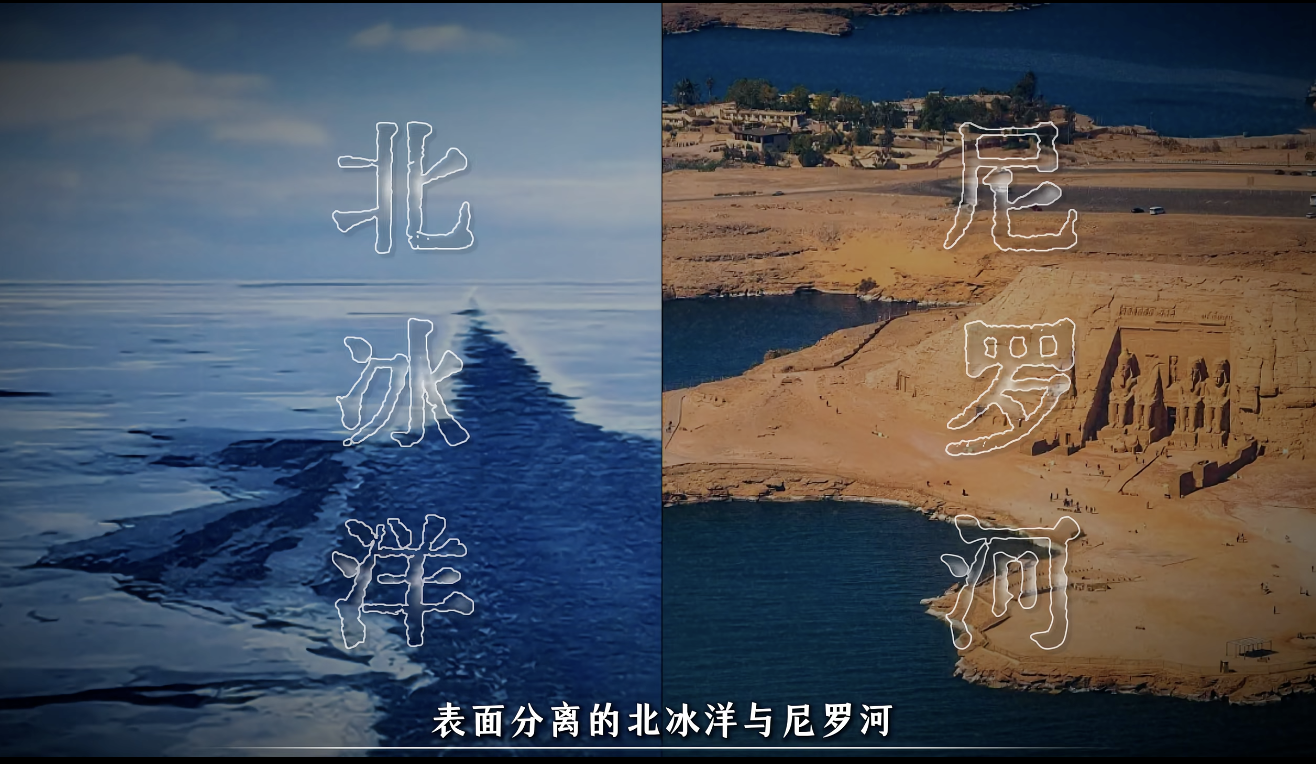
\includegraphics[width=\linewidth]{image/黑塞的水1.png}
        \caption{万物归一示意图}
        \label{fig:water1}
    \end{subfigure}
    \hspace{2em}   % 固定间距，替代 \hfill
    \begin{subfigure}[b]{0.42\textwidth}
        \centering
        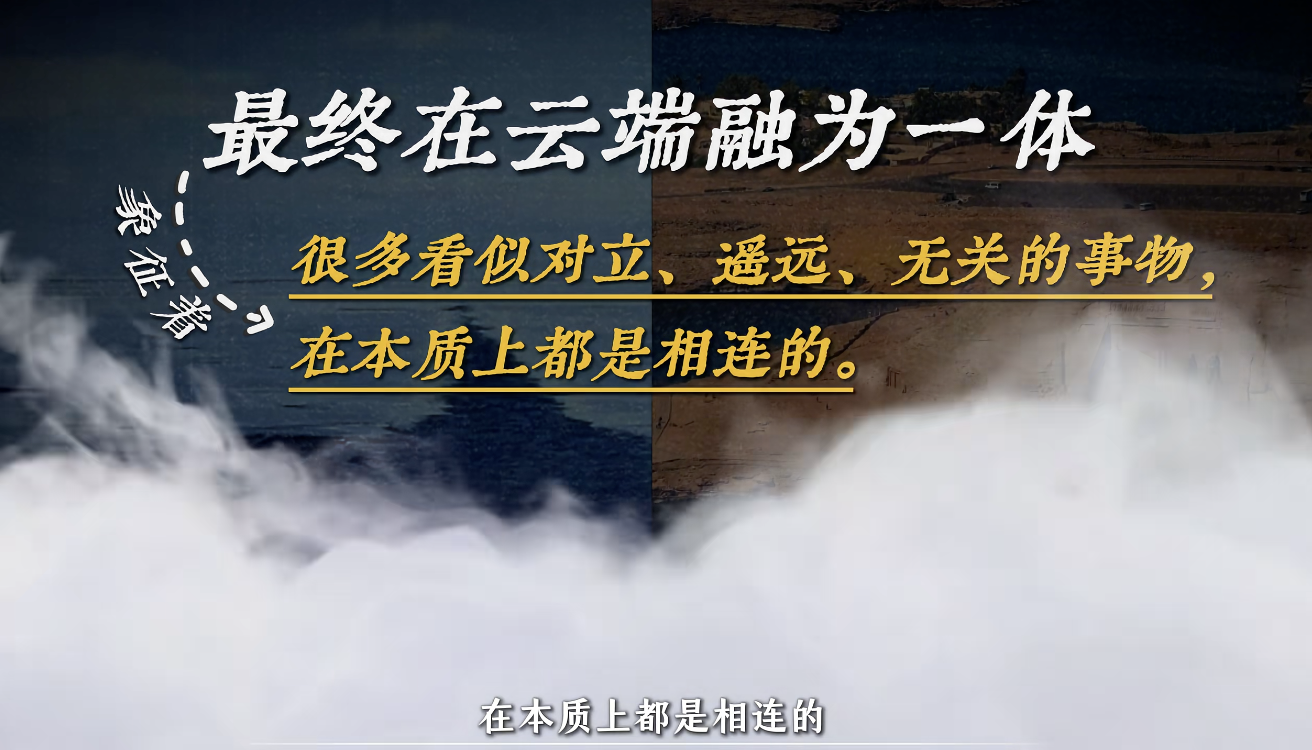
\includegraphics[width=\linewidth]{image/黑塞的水2.png}
        \caption{循环往复示意图}
        \label{fig:water2}
    \end{subfigure}
    \caption{水的哲学意象}
    \label{fig:waters}
\end{figure}


\section{第一组：成长感悟类——引用黑塞名言的写作思路}

\noindent \textbf{通用策略：} 将“水”作为贯穿全文的核心意象（雨、溪流、海、云、眼泪等），在关键转折处点明“水”与“重逢”的关系，结尾直接化用或引用黑塞原句。



\subsection{一、《那一刻，我读懂了\_\_》}

\textbf{题目解读：} 强调从“不懂”到“懂”的瞬间顿悟。适合写亲情、友情、师长教诲、艺术欣赏、自然启示等。

\textbf{引用思路：}
\begin{itemize}
    \item 将“读懂”视为水的“交汇”——曾互不相解，在特殊时刻两条河流在湿云中交融。
    \item 将“那一刻”比作水循环的“蒸发—凝结”节点——困惑升腾为顿悟，再落回清澈。
\end{itemize}

\textbf{写作提纲：}
\begin{enumerate}
    \item \textbf{开头：} 以水的意象引出“不解”，如“我曾以为我和父亲就像两条永不交汇的河。”
    \item \textbf{主体：} 描述“不懂”的日常，然后描写“那一刻”的具体事件，融入雨、泪、汗等水元素。
    \item \textbf{转折：} 瞬间“读懂”，悟到对方的沉默也是另一种流淌。
    \item \textbf{结尾：} “如今我相信，北冰洋与尼罗河会在湿云中交融，而我和父亲，也终于在那一刻读懂了彼此的流向。”
\end{enumerate}

\textbf{示例结尾：}“那一刻，窗外的雨滴连成线，我的泪水也滑落。原来不是所有的爱都要喧哗，有些深流藏在水面之下。就像黑塞说的，北冰洋与尼罗河会在湿云中交融，而我与父亲，也终于在那一刻，读懂了彼此沉默的河床。”



\subsection{二、《这样的挫折让我成长》}

\textbf{题目解读：}强调挫折与成长的因果，需写出具体挫折、内心挣扎和最终收获。

\textbf{引用思路：}
\begin{itemize}
    \item 挫折比作水流的迂回或坠落，但不会停止，最终流向大海。
    \item 成长视为循环——低谷蕴含上升的种子。
    \item 殊途同归——所有弯路终将指向真实自我。
\end{itemize}

\textbf{写作提纲：}
\begin{enumerate}
    \item \textbf{开头：} “我曾以为人生应如直下的瀑布，直到我跌入暗流。”
    \item \textbf{主体：} 叙述一次具体挫折（考试、比赛、人际等），融入汗水、泪水、暴雨等水意象。
    \item \textbf{转折：} 在挫折中找到方法，意识到这是“转弯”而非终点。
    \item \textbf{结尾：} “北冰洋的冰不是结束，是它奔赴尼罗河的前奏。所有的挫折都像水流的低洼，为了在更高的云端与成功重逢。”
\end{enumerate}

\textbf{示例结尾：}“那次失利后，我曾以为我的河流彻底干涸。但时间告诉我，水从未消失，它只是渗入地下，去往另一片海。正如黑塞所写，全世界的水都会重逢，失败与成功也会在生命的云图中交融。这样的挫折，原来是为了让我成长得更深、更阔。”


\subsection*{三、《藏在\_\_里的蜕变》}

\textbf{题目解读：}强调变化发生于隐秘之处、经过时间的酝酿，适合写内在品质、技艺或情感成熟。

\textbf{引用思路：}
\begin{itemize}
    \item 蜕变比作水循环的形态变化——水“藏”入天空，看不见，但最终以雨降落，焕然一新。
    \item “藏”的过程比作地下暗流，默默滋养。
    \item 殊途同归——蜕变前的迷茫和积累，终将汇入更阔的生命之海。
\end{itemize}

\textbf{写作提纲：}
\begin{enumerate}
    \item \textbf{开头：} “我曾以为那些灰暗的练习时光一文不值，它们只是藏在角落里。可后来我才明白，那里正进行着一场水的蜕变。”
    \item \textbf{主体：} 描写“藏”的阶段——重复、枯燥、孤独的努力，细节扎实，隐喻为水在地下渗透。
    \item \textbf{转折：} 默默积累突然显现成果（登台、发表等），蜕变完成，如一滴水升腾成云被阳光照亮。
    \item \textbf{结尾：} “原来，每一滴水的旅程都不是徒劳。藏在暗处的水汽，终将在湿云中与万千水滴相聚，化作彩虹。”
\end{enumerate}

\textbf{示例结尾：}“那些藏在深夜里的反复演练，那些不为旁人所知的咬牙坚持，都像是水在暗处的蒸腾。没有人看到它们，但它们确确实实地上升、汇聚。直到某天，云开雨落，全世界的水都重逢——原来我的蜕变，也是一场北冰洋与尼罗河的遥远合谋。”


\subsection*{四、《为了心中的那束光》}

\textbf{题目解读：}“那束光”象征目标、理想、信念或重要的人，需突出追求过程中的困难与执着。

\textbf{引用思路：}
\begin{itemize}
    \item 将“光”与“水”融合——追求者如朝光蒸腾的水，最终在光中化为云霞。
    \item 循环往复诠释坚持——每一次向光靠近都可能遇到暗礁，但水相信终将与光重逢。
    \item 万物归一——所有努力终将指向那束光，如不同河流归于大海。
\end{itemize}

\textbf{写作提纲：}
\begin{enumerate}
    \item \textbf{开头：} 直接点明“光”，并用水的意象引入：“我是一滴水，心中却藏着一片海洋，而那片海洋的名字，就是远方的那束光。”
    \item \textbf{主体：} 叙述追寻光的过程中的困难、诱惑、犹豫，穿插汗、雨、泪等水元素。
    \item \textbf{转折：} 低谷时，光依然在远方或突然变亮，激励前行。
    \item \textbf{结尾：} “我相信，只要不放弃流动，每一滴水都能抵达光的怀抱。北冰洋与尼罗河在湿云中交融，而我心中的那束光，也终将与我所有的汗水、泪水在云端相拥。”
\end{enumerate}

\textbf{示例结尾：}“为了那束光，我流过干旱的沙漠，也经过严寒的冰原。但我记得黑塞的话——全世界的水都会重逢。光与水本就是一体，当我终于蒸腾成云，那束光穿透我的身体，我便成了朝霞。原来，为了心中的那束光而奔跑，就是让一滴水找到自己的星空。”


\section{通用化用要点}
\begin{tcolorbox}[colback=yellow!10, colframe=orange!50, title=化用要点]
\begin{enumerate}[leftmargin=*]
    \item \textbf{铺垫要自然：} 前文至少出现一次与“水”相关的意象（雨、海、汗、泪、溪流等），使结尾的名言不突兀。
    \item \textbf{不必全句照搬：} 可拆解为“北冰洋的寒流”“尼罗河的暖”“湿云”“重逢”等碎片，穿插在叙事中。
    \item \textbf{避免说教：} 哲理要通过故事本身渗透，而不是直接喊口号。
    \item \textbf{保持真诚：} 所写事件必须真实或可信，否则名言的厚重感会被削弱。
\end{enumerate}
\end{tcolorbox}


\section{坚持}


坚持开头:“不积跬步无以至千里，不积小流无以成江海”没有一蹴而就的胜利，只有厚积薄发的坚持。坚持不一定能成功，但坚持能够让我们对生命和未来仍有所期待。

结尾：“古之成大事者不惟有超世之才，亦必有坚韧不拔之志”平坦的康庄大道，不需要坚持。崎岖的蜿蜒小路，才是命运对你的考验。再坚持一下，是一种信念，也是一种转机。


\section{幸好有苏试}


\begin{tcolorbox}[colback=blue!5, colframe=blue!50, title=主题一：旷达乐观的处世哲学]
适用场景：面对人生风雨、逆境与挑战时的态度。
素材支撑：乌台诗案后被贬黄州，苏轼并未沉沦。他脱下长衫开荒种地，自号“东坡居士”；买不起羊肉便发明“东坡肉”；雨中穿林打叶，依然能吟出“一蓑烟雨任平生”。 他的乐观是将绝境活成生活美学。
\end{tcolorbox}

\begin{tcolorbox}[colback=green!5, colframe=green!50, title=主题二：坚韧不拔的生命韧性]
适用场景：讨论坚持、生命力、在困苦中成长。
素材支撑：晚年被贬至当时被视为绝境的海南儋州，60多岁的苏轼没有等死，而是 在当地办起学堂亲自讲学，培养出海南历史上第一位举人 。他将个人苦难转化为泽被苍生的行动。
\end{tcolorbox}

\begin{tcolorbox}[colback=orange!5, colframe=orange!50, title=主题三：破茧成蝶的思想格局]
适用场景：谈格局、放下个人恩怨、精神境界。
素材支撑：苏轼能跳出二元对立的局限。最典型的是，他虽与王安石政见不合，但在王安石罢相后主动拜访，两人同游中山、谈诗论道， 留下“相逢一笑泯恩仇”的佳话 。
\end{tcolorbox}


\subsection{幸好有苏轼}

文字，是两个灵瑰交流最直接的方式。
——题记

又是一个"不眠之夜"！
望着铺天盖地的试卷，透过窗户的反光，我看到一个憔悴的自己。压力如石的初三，盲目努力而未得回报，我身处黑暗，内心充满绝望和不甘。
我打开窗户，清冷的风灌了进来，我又随手打开了摘抄本。

"竹杖芒鞋轻胜马，谁怕？一蓑烟雨任平生"映入眼帘，我被这些文字吸引，进入了苏轼的时空。

寒风仍在吹，有雨，还有一个吟咏长啸、悠然自得的诗人，即使是竹杖芒鞋行走在泥泞之中也毫不在意，反而仰面朝天，任凭雨点打落，他是那么从容不迫，眼角有笑意，眼中有深意。"归去，也无风雨;也无晴"，他豁达大度，我疑惑，明明有风雨，为何他却说"也无风雨也无睛"？还没缓过神来，他继续说道："人生几时欢喜几时愁，雨后仍是晴空，我东坡的一生，有得意有坎坷，归来，心中仍怀大志！"
寒风又灌了进来，回过神，我想起苏轼在《自题金山画像》中写到的那甸"问汝平生功业，黄州惠州儋州"，虽有自嘲的意味，但也写出了贬谪生涯在他一生中的重要位置。也许正是仕途中的低谷，成就了他思想、性格、心态上的乐观豁达，乃至文学上的高峰。那我今天的低谷又算得了什么呢？我释然一笑，打开了那份沉重的成绩单，"人有悲欢离合，月有阴晴圆缺"，只要我心向阳，又怎会怕眼前短暂的黑暗呢？

目光又被另一句诗吸引："粗缯大布裹生涯，腹有诗书气自华。"一个身着布衣、朴实无华的诗人再次出现在我眼前，他手握诗卷，望向远方，他领悟人生于心中，寄托情怀于诗书里。

我如梦初醒，幸好有苏轼。他引导我走出黑暗，他引导我在乐观向上的人生道路上前行，他引导我在文字中领悟诗意之美。

、幸好有苏轼。我在摘抄本上写下：无论雨，无论睛，腹有诗书，文笔留韵。
这，无疑是一场我与东坡通过文字进行的灵魂交流。——后记


\chapter{写作XX}


\section{写作（50分）}

阅读下面的文字，根据要求写作。（50分）

并非站在山顶，才能被看见。

以上文字引发了怎样的联想和思考？请联系自己的生活经历和感受，写一篇文章。


凡人微光

\chapter{考场练兵答案}

\section{选择}

\paragraph{1.} 答案：C

解析：A. 语序不当，改为：既影响了汉语表意功能的发挥，也消解了中国文化精深而丰富的内涵；B. 两面对一面，去掉“能否”或在“在于”后加上“能否”；D. 关联词语使用不当，改“尽管”为“不管”。

% 第2题
\paragraph{2.} 答案：B

解析：B. 成分残缺，应在“环境保护”后加上“力度”。

% 第3题
\paragraph{3.} 答案：B

解析：B. 搭配不当。“效率”与“改动”“改变”都不能搭配，应将“改动”改为“提高”。

% 第4题
\paragraph{4.} 答案：C

解析：C. “该句有语病，应把‘提升’改为‘提高’”有误，“提升了民族文化的交流”搭配不当，应把“提升”改为“促进”。

% 第5题
\paragraph{5.} 答案：B

解析：A. 语序不当，将“我们”放在“只有”前；C. 否定不当，删去“不再”；D. 搭配不当，将“表示”改为“表达”。


\section{阅读}

\begin{enumerate}[leftmargin=*]
    \item （1）fēng ráo \quad （2）污秽
    \item （3）C \quad （4）A \quad （5）B
    \item B
    \item 夜夜我听见马蹄奔驰的声音，草原的儿子在黎明的天边呼唤。
\end{enumerate}

解析：

\subsection*{（1）}
\begin{itemize}[leftmargin=*]
    \item 丰饶（fēng ráo）：丰裕富饶；丰足充实。
    \item 污秽（wū huì）：肮脏的；不洁净的（物体）。
\end{itemize}

\subsection*{（2）}
\begin{itemize}[leftmargin=*]
    \item 谦逊：谦虚、不浮夸，不自大或不虚夸。
    \item 宽广：面积大，宽阔。
    \item 坚韧：指物体坚固而柔韧，不容易折断；指人的性格品质不屈不挠，意志坚定，坚忍有韧性。
\end{itemize}

第一空：在此形容意志，应用“坚韧”，故选 C。\\
第二空：在此形容气质，应用“谦逊”，故选 A。\\
第三空：在此形容胸怀，应用“宽广”，故选 B。

\subsection*{（3）}
本题考查词性。

B.“他们看来是很平凡、很简单的哩”中的“很”是副词；故选 B。

\subsection*{（4）}
本题考查病句修改。

“看见”与“声音”搭配不当，应将“看见”改为“听见”。





\chapter{考试范围}


第1--6单元 + 名著《骆驼祥子》《钢铁是怎样炼成的》，覆盖基础、阅读、写作三大板块，按考查权重排序。附：必背要点与答题模板，适配所有部编版教材，七年级下册通用。

\section*{一、语言积累与运用（25--30分，基础必拿分）}

\subsection*{1. 字音字形（8--10分）}

\textbf{高频易错字：}

\begin{itemize}[leftmargin=*]
    \item \textbf{第一单元：} 殷（yān）红、卓（zhuó）越、鞠（jū）躬尽、锲（qiè）而不舍、锋芒毕露、至死不懈、家喻户晓
    \item \textbf{第二单元：} 哺（bǔ）育、澎湃（pài）、澜（lán）语、默契（qì）、浩浩荡荡
    \item \textbf{第三单元：} 憎（zēng）恶、区（ōu）楼、滞（zhì）留、颔（hàn）头、取缔（dì）、烦躁（zào）
    \item \textbf{第四单元：} 崎岖（qí qū）、噩耗（è hào）、毛坯（máo pī）、辗转难眠（zhǎn zhuǎn nán mián）
    \item \textbf{第五单元：} 深坳（shēn ào）、梭镖（suō biāo）、砍伐（kǎn fá）、摇撼（yáo hàn）
    \item \textbf{第六单元：} 合拢（hé lǒng）、吟唱（yín chàng）、孤零零（gū líng líng）、不期而至（bù qī ér zhì）、心有灵犀（xīn yǒu líng xī）
\end{itemize}

\textbf{多音字：} 调（diào/tiáo）、强（qiáng/qiǎng/jiàng）、塞（sāi/sè/sài）

\textbf{字形辨析：} 辨清“躁/燥/澡”“概/慨”“即/既”“辨/辩”，重点防范成语写错字。

\subsection*{2. 古诗文默写（6--8分）}

\textbf{必背篇目：} 《竹里馆》《春夜洛城闻笛》《晚春》《逢入京使》《孙权劝学》（重点句子）、《卖油翁》（重点句子）

\textbf{高频默写句（必背，杜绝错别字）：}

\begin{itemize}[leftmargin=*]
    \item \textbf{《竹里馆》：} 独坐幽篁里，弹琴复长啸。深林人不知，明月来相照。
    \item \textbf{《春夜洛城闻笛》：} 谁家玉笛暗飞声，散入春风满洛城。此夜曲中闻折柳，何人不起故园情。
    \item \textbf{《晚春》：} 草树知春不久归，百般红紫斗芳菲。杨花榆荚无才思，惟解漫天作雪飞。
    \item \textbf{《逢入京使》：} 故园东望路漫漫，双袖龙钟泪不干。马上相逢无纸笔，凭君传语报平安。
    \item \textbf{《孙权劝学》：} 卿今当涂掌事，不可不学！但当涉猎，见往事耳；士别三日，即更刮目相待。
\end{itemize}

\textbf{易错字：} 篁、折柳、涉猎、卿、涂、荚、惟、龙钟

\subsection*{3. 文学常识与名著（5--7分）}

\textbf{文学常识：}

\begin{itemize}[leftmargin=*]
    \item （1）\textbf{《资治通鉴》：} 北宋司马光主持编纂的编年体通史，记载了从战国到五代共1362年的历史。
    \item （2）\textbf{《木兰诗》：} 南北朝时期北方乐府民歌，与《孔雀东南飞》并称“乐府双璧”，收录于《乐府诗集》。
    \item （3）\textbf{重点作者及作品：} 杨振宁《邓稼先》、臧克家《说和做——记闻一多先生言行片段》、陆定一《老山界》、鲁迅《阿长与〈山海经〉》、欧阳修《卖油翁》。
\end{itemize}

\textbf{名著《骆驼祥子》（必考，重点掌握）：}

\begin{itemize}[leftmargin=*]
    \item （1）\textbf{作者：} 老舍，原名舒庆春，字舍予，现代著名作家，被授予“人民艺术家”称号。
    \item （2）\textbf{核心人物：} 祥子（前期：勤劳、朴实、坚韧、有梦想；后期：麻木、潦倒、自私、堕落）、虎妞（泼辣、霸道、贪婪）、刘四爷（残忍、自私、吝啬）。
    \item （3）\textbf{核心情节（三起三落，必考）：}
        \begin{itemize}
            \item 一起：祥子苦干三年，攒钱买了一辆新车；
            \item 一落：新车被大兵抢走，祥子沦为乞丐；
            \item 二起：祥子重新攒钱，准备买新车；
            \item 二落：攒下的钱被孙侦探敲诈一空；
            \item 三起：虎妞出钱，给祥子买了一辆二手车；
            \item 三落：虎妞难产而死，祥子卖掉二手车安葬虎妞，彻底沦为行尸走肉。
        \end{itemize}
    \item （4）\textbf{主题：} 揭露旧社会对底层劳动者的残酷压迫，批判黑暗、腐朽的社会制度，表达对底层人民的同情。
\end{itemize}

\textbf{名著《钢铁是怎样炼成的》（必考，重点掌握）：}

\begin{itemize}[leftmargin=*]
    \item （1）\textbf{作者：} 苏联奥斯特洛夫斯基，自传体长篇小说，全身瘫痪、双目失明后完成创作。
    \item （2）\textbf{核心人物：} 保尔（主角，意志坚定、顽强不屈、无私奉献，为人类解放事业奋斗终身）、朱赫来（保尔革命引路人，布尔什维克党员，教会保尔革命道理）。
    \item （3）\textbf{关键情节（填空/简答）：}
        \begin{itemize}
            \item 四次死里逃生：与波兰白军战斗，腿伤+伤寒；骑兵战头部重伤，右眼失明；肃反工作积劳成疾；筑路时患伤寒+大叶性肺炎。
        \end{itemize}
    \item （4）\textbf{保尔精神：} 为理想献身、坚韧不拔、顽强奋斗、无私奉献。
\end{itemize}

\subsection*{4. 词语运用（4--6分）}

\begin{itemize}[leftmargin=*]
    \item \textbf{成语辨析：} 重点掌握“锲而不舍、兀兀穷年、沥尽心血、家喻户晓、鲜为人知、可歌可泣、深恶痛绝、微不足道”，结合语境判断使用正误。
    \item \textbf{词语语境义：} 如“涉猎”（粗略阅读）、“刮目相待”（用新的眼光看待）、“微不足道”（非常渺小，不值得一提）。
\end{itemize}

\subsection*{5. 病句辨析与修改（3--4分）}

\textbf{高频病句类型：} 成分残缺、搭配不当、语序不当、前后矛盾、表意不明、重复累赘。

\textbf{典型示例及修改：}

\begin{enumerate}[leftmargin=*]
    \item 错误：通过开展“书香校园”活动，使同学们的阅读水平有了明显提高。\\
    修改：删去“通过”或“使”，补充主语。
    \item 错误：我们要养成认真完成作业的好习惯和态度。\\
    修改：删去“和态度”，搭配不当。
    \item 错误：他经常回忆过去的往事。\\
    修改：删去“过去的”或“往”，重复累赘。
\end{enumerate}

\section*{二、文言文阅读（12--15分，2篇：课内1篇+课外1篇）}

\subsection*{课内必考（考查概率90\%，重点突破）}

\subsubsection*{《短文两篇》——《陋室铭》}

\begin{table}[h]
\centering
\begin{tabular}{|m{4cm}|m{10cm}|}
\hline
\textbf{考查类型} & \textbf{具体内容} \\
\hline
词类活用 & 名、灵、馨、乱、劳、上 \\
\hline
古今异义 & 形、馨、鸿、丝竹、调（90\%学生混淆“鸿”的古今含义） \\
\hline
\multirow{5}{*}{重点句子翻译} & 1. 斯是陋室，惟吾德馨。 \\
 & 2. 苔痕上阶绿，草色入帘青。 \\
 & 3. 谈笑有鸿儒，往来无白丁。 \\
 & 4. 可以调素琴，阅金经。 \\
 & 5. 无丝竹之乱耳，无案牍之劳形。 \\
\hline
\end{tabular}
\end{table}



\end{document}
